\section{Klassifizierung}
\script{135} Das einfachste Klassifierungsproblem (Zwei Klassen) kann zB durch das Modell
\[
p(x) = \frac{e^{\beta_0 + \beta_1x}}{1+ e^{\beta_0 + \beta_1x}}
\]
abgebildet werden. Der Ausgang sagt, mit welcher Wahrscheinlichkeit ein $x$ zur Klasse 0 oder 1 gehört.

\subsection{LDA}
Linear Discrominant Analysis maximiert die Distanz von $\mu_k$, dem Durchschnitt der jeweiligen Klasse und die Varianz auf der proijezierten Achse.
\begin{center}
	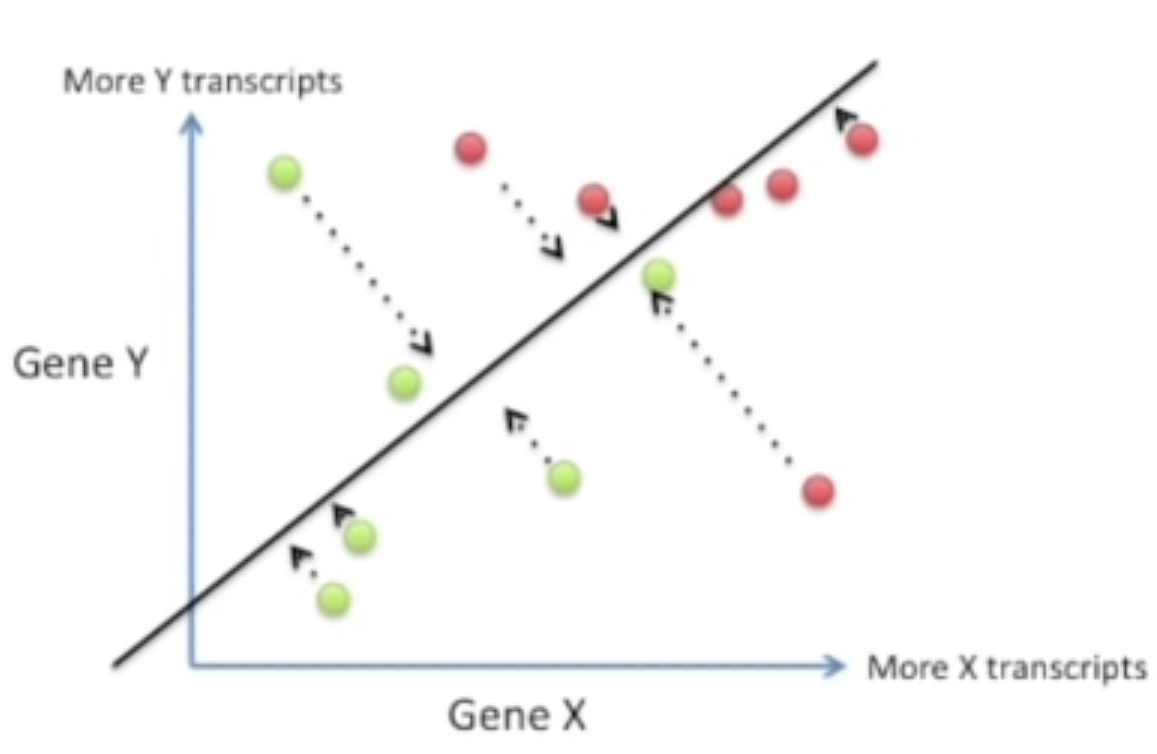
\includegraphics[width=0.8\columnwidth]{./Images/lda}
\end{center}

Die dazu notwendigen Parameter für LDA mit $p=1$ ($K$ Klassen, $n_k$ Anzahl pro Klasse und $n$ Sampels) sind $\hat{\pi}_k$ und $\hat{\sigma}^2$.

\begin{align*}
	\hat{\mu}_k &= \frac{1}{n_k}\sum_{i: y_i=k} x_i \qquad \text{Durchschnitt pro Klasse} \\
	\hat\sigma^2 &= \frac{1}{n-K}\sum_{k=1}^{K}\sum_{i: y_i=k}(x_i-\hat\mu_k)^2
\end{align*}

Die Prior Probability ist gegeben durch $\hat{\pi}_k = \frac{n_k}{n}$. Damit lässt sich nun die Achse für jede Klasse beschreiben:
\[
\hat\delta_k(x) = x \cdot \frac{\hat\mu_k}{\hat\sigma^2}-\frac{\hat\mu_k^2}{2\hat\sigma^2} + \log{\hat\pi_k}
\]

Für $p\gt1$ siehe \script{142} und statt $\sigma^2$ wird eine Covarianz Matrix $\Sigma$ verwendet.